\section{3D Map preprocessing}
Since smaller volumes usually include lower number of individual structural elements, making easier fitting models in maps and simplifying modeling process, the volume chosen will always be the smaller asymmetrical subunit of the starting loaded volume, also known as unit cell. The size of the unit cell thus depends on the symmetry order of the initial volume. The higher the symmetry order, the smaller the unit cell. The atomic structure of the whole volume will be obtained straight forward by simply repetition of the unit cell structure according to the symmetry. Then, the first step to simplify the complexity of the initial volume is extracting the unit cell. This task can be accomplished by using the \scipion protocol \scommand{extract unit cell}. 

\ffigure{fig:extract_unit_cell} shows how to fill in this protocol form (1). Since \ttt{metHgb} macromolecule shows symmetry C2, we have selected cyclindric symmetry (Cn) as type of symmetry, and 2 as symmetry order. The angle offset selected (-45º) turns around the z axis the mask used to create the unit cell. 
%Remark the relevance of including the offset in order to extract a unit cell able to reconstruct by symmetry the whole volume regarding the symmetry axes. 
The extracted fraction of the initial volume will include the volume comprised between the coordinate origin (inner radius 0.0) and the maximum radius (outer radius 50.0), and will be slightly higher than the unit cell (expand factor 0.2). % We use an expanded unit cell  to favor the modeling of each individual structure edges. 
Again, the respective tutorial appendix \ref{app:extractUnitCell} includes a comprehensive explanation of the meaning of parameters. 

 \begin{figure}[H]
  \centering 
  \captionsetup{width=.7\linewidth} 
  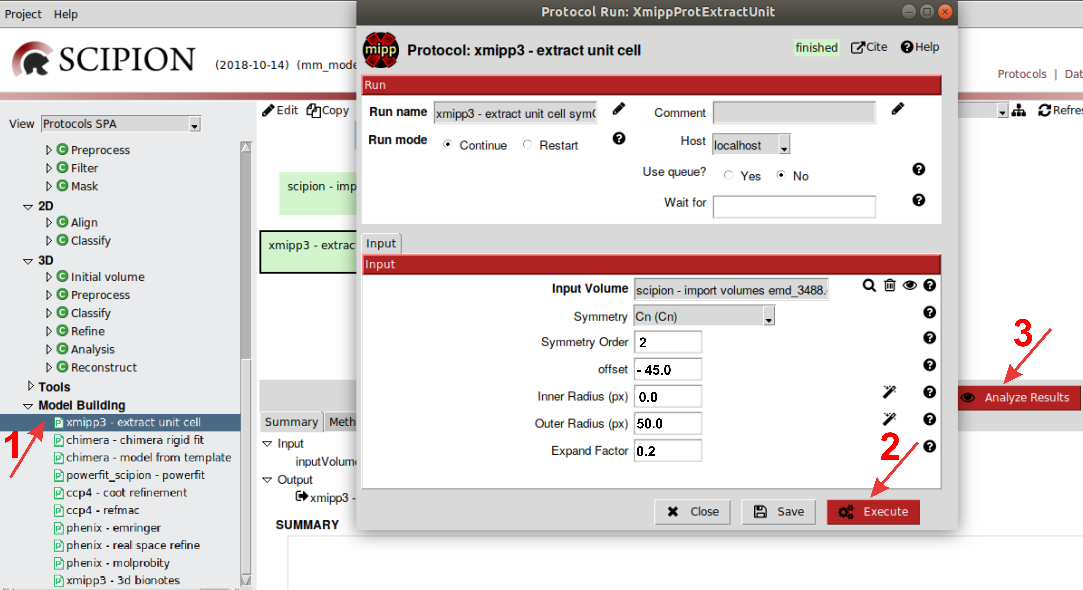
\includegraphics[width=0.90\textwidth]
  {Images/Fig7}
  \caption{Extracting the unit cell volume.}
  \label{fig:extract_unit_cell}
  \end{figure}
  
After executing the protocol (\ffigure{fig:extract_unit_cell}(2)), the resulting expanded unit cell can be observed (3) with \chimera (\ffigure{fig:chimera_visualization_unit_cell}). Note the additional expanded volume of the  unit cell on the left side of the figure. The unit cell itself, on the right side, constitutes the half volume. Since the total volume contains the structure of four proteins, we can predict that this smaller asymmetrical subunit of the initial volume contains two proteins, one $\alpha$ and one $\beta$ \ttt{metHbg} subunits. Then, the respective structures of these two proteins will be fitted in the unit cell volume in successive modeling workflow steps. 
  
 \begin{figure}[H]
  \centering 
  \captionsetup{width=.7\linewidth} 
  \includegraphics[width=0.80\textwidth]
  {Images/Fig8}
  \caption{Expanded unit cell (green-blue) and initial volume (gray) visualized with $Chimera$. The purple broken line delimits the unit cell (right) and its expanded volume (left).}
  \label{fig:chimera_visualization_unit_cell}
  \end{figure}
